%% Load document class fithesis2
%% {10pt, 11pt, 12pt}
%% {draft, final}
%% {oneside, twoside}
%% {onecolumn, twocolumn}
\documentclass[12pt,final,oneside]{fithesis2}

%% Basic packages
\usepackage[english]{babel}
\usepackage{cmap}
\usepackage[T1]{fontenc}
\usepackage{lmodern}
\usepackage[utf8]{inputenc}
\usepackage{graphicx}

%% Additional packages for colors, advanced
%% formatting options, etc.
%\usepackage{color}
%\usepackage{microtype}
\usepackage{url}
%\usepackage{cslatexquotes}
%\usepackage{fancyvrb}
%\usepackage[small,bf]{caption}
\usepackage[plainpages=false,pdfpagelabels,unicode]{hyperref}
%\usepackage[all]{hypcap}

\usepackage{amsmath}
\usepackage{amsfonts}
\usepackage{amsthm}

\theoremstyle{definition}
\newtheorem{definition}{Definition}

\usepackage{listings}

\lstset{
    basicstyle=\small\ttfamily,
    captionpos=b
}

\usepackage{tikz}

\newcommand\emptypage{\newpage\null\thispagestyle{empty}\newpage}

\setcounter{tocdepth}{3}

%% Fix long URLs in DVIs
%\usepackage{ifpdf}

%\ifpdf
%\else
%  \usepackage{breakurl}
%\fi

%% Packages used to generate various lists
%\usepackage{makeidx}
%\makeindex

%\usepackage[xindy]{glossaries}
%\makeglossary

%% Use STAR and CIRCLE signs for nested
%% itemized lists
%\renewcommand{\labelitemii}{$\star$}
%\renewcommand{\labelitemiii}{$\circ$}

%% Title page information
\thesistitle{String abstract domains}
\thesissubtitle{Master's thesis}
\thesisstudent{Bc. Matej Šuta}
\thesiswoman{false} %% Important when using Slovak or Czech lang
\thesisfaculty{fi}  %% {fi, eco, law, sci, fsps, phil, ped, med, fss}
\thesislang{en}     %% {en, sk, cs}
\thesisyear{Spring 2013}
\thesisadvisor{Mgr. Karel Klíč}

%% Beginning of the document
\begin{document}

%% Front page with a logo and basic thesis information
\FrontMatter
\ThesisTitlePage

\emptypage

%% Thesis declaration (required)
\begin{ThesisDeclaration}
  \DeclarationText
  \AdvisorName
\end{ThesisDeclaration}

%% Thanks (optional)
\begin{ThesisThanks}
My thanks go to my thesis supervisor Karel Klic, my colleagues in his
study group Jan Dupal and Tomas Brukner and all the people who
supported me during the writing of this thesis.
\end{ThesisThanks}

%% Abstract (required)
\begin{ThesisAbstract}
This thesis is about ...
\end{ThesisAbstract}

%% Keywords (required)
\begin{ThesisKeyWords}
static analysis, abstract interpretation, abstract domain, string,
prefix, suffix, trie
\end{ThesisKeyWords}

%% Beginning of the thesis itself
\MainMatter

%% TOC (required)
\tableofcontents


\chapter{Introduction}

Computers have followed Moore's~law~\cite{Moore65-1} for more than
four decades now. Hardware gets more powerful and complex. Consequently,
this results in software being more complex too. It has to be designed
with maintainability and reliability in mind. Therefore several software
verification methods have been created. Abstract interpretation is one
of them.

There are many aspects of a computer program that may be analyzed by
abstract interpretation. The focus of this thesis is how program manipulates
strings. A string is very flexible data structure that allows programmer
to represent practically anything. In fact, most of the programs written
today have to deal with strings in some form. Thus, it is important to know
how programs treat strings.

This thesis describes string abstract domains in context of abstract
interpretation framework. It is based on papers published
by Cousot~\cite{CousotCousot77-1} and other authors. The goal of the thesis
is to design, implement and integrate several abstract domains for strings
into \texttt{canal} abstract interpreter. \texttt{canal} is a tool designed
to analyze behavior of application programs written in \texttt{C}.

The text has the following outline: chapter~\ref{chap:preliminaries}
presents preliminaries required to understand the abstract interpretation.
In chapter~\ref{chap:design} several string abstract domains are designed.
The implementation of designed domains is described in great detail in
chapter~\ref{chap:implementation}. Finally, thesis findings are summarized
in chapter~\ref{chap:conclusion}. Appendix~\ref{chap:instructions} contains
instructions for compiling and running the \texttt{canal} abstract
interpreter.


\chapter{Static analysis and abstract interpretation}
\label{chap:preliminaries}

The notion of quality is an abstract concept. In software engineering it
represents a multi-aspect property of a product which includes but is not
limited to characteristics such as stability, maintainability, realiability,
efficiency or security. It plays an important role in recognition of
particular software.

It is certainly true that not every project needs to have as high quality as
safety critical systems but to a certain degree quality matters
everywhere. It is crucial for software maintainability which becomes
especially difficult when size of a codebase and number of developers
increases. This chapter describes various techniques used to
improve these properties and abstract interpretation in particular.


\section{Software quality evaluation techniques}

Traditionally the set of quality control techniques are referred to as
validation and verification. According to
Boulanger~\cite{Boulanger12-1} these terms are defined in standard
ISO 9000:2000 as:

\begin{description}

\item[Verification] \hfill \\
confirmation by tangible proof that the specified requirements have
been met at each stage of the realization process

\item[Validation] \hfill \\
confirmation by tangible proof that the requirements for a specific use or
an anticipated application have been met

\end{description}

Applied in software engineering the definitions above summarize the
processes that ensure and demonstrate that the resulting software product
achieves the desired quality level.

The validation is usually performed by executing a program with intention
to assure that the software product meets the requirements of a customer.
The process can be manual or completely automatic. It includes
various types of tests such as acceptance testing, performance testing,
penetration testing, etc. Functional testing consists of test cases
being executed to check various scenarios and is traditionally performed
by quality assurence specialist. Main benefit of testing is that the
application is run under real confitions and the specialist is able to
check the presence of yet unidentified errors. The output of the validation
is statement whether the built solution is the right one.

The verification may be done either by executing the program or by
analyzing the source code of the program. They are called \textit{dynamic}
and \textit{static} verification respectively. These activities are
typically performed by a programmer during the development phase.
There are many disciplines that enforce the verification by program
execution -- unit testing or integration testing among others. These
disciplines are relatively easy to understand and implement. The main
disadvantages include testing in isolation. In addition, this type of
testing can only check for presence of known errors. The static
verification usually includes source code inspection either manually or
by a tool. Implementation of such tool usually requires a deep
theoretical knowledge and programming skills.

Note that it is possible for program to pass the verification and
fail the validation step, hence the realationship between the approaches
should complementary rather then contradictory in order to achieve the
highest possible quality. Moreover, there is no
precise distinction between the two. Test driven development or behavior
driven development are two examples of techniques which perform
verification by executing unit tests and also validate that requirements
have been met.


\section{Static analysis}

Static code analysis is a well known term in software industry yet there
is a lot of confusion surrounding it. Emanuelsson and Nilsson
\cite{EmanuelssonNilsson08-1} refer to it as the analysis of a computer
program without actually executing it. This process is fully automatic
but a programmer needs to interpret the results of analysis and make
proper adjustments to the analyzed code.

Most of the languages do not have a support for runtime error detection.
It is programmers responsibility to ensure these errors do not occur
and deal with them once they do. The errors do not include simple type
checking or syntax errors although even these could be considered a part
of static analysis. They are already checked by compiler. Hence, only
errors which lead to unexpected or undefined behavior are checked.
Consider the \texttt{C} code in listing~\ref{lst:outofbounds}:

\begin{lstlisting}[
    language=C,
    caption={Out of bounds array access},
    label=lst:outofbounds
]

    int array[3] = { 1, 2, 3 };
    int value = array[3];

\end{lstlisting}

In the example the \texttt{array} variable contains three integers but
\texttt{value} variable will contain unexpected value because it is
accessing the fourth element of the \texttt{array}. Moreover, the
listing will compile and run, but the number might be different every
time the program is run since accessing the items out of array bounds is
undefined behavior in \texttt{C} programming language. Other typical
examples of errors potentially detected by static analysis could be
division by zero or infinite loops.

The applications of static analysis are quite extensive as it has been
shown by Emanuelsson and Nilsson \cite{EmanuelssonNilsson08-1}. Besides
already mentioned examples and out of bounds array acces demonstrated in
listing \ref{lst:outofbounds} it is possible to check:

\begin{itemize}

\item Initialization of pointers, variables and return values --
manipulating uninitialized values can produce runtime errors

\item Operations with numerical types -- adding two big numbers may lead
to overflow of the datatype

\item Pointer arithmetics -- check the incorrect pointer handling which
can generate segmentation faults or memory corruption

\item Function invocation -- calling a function with incorrect argument
properties can cause undefined behavior e.g. calling square root
function with negative number

\item Unreachable or dead code -- verification of the data flow and
branching of the code within the program

\item Memory management -- check that the memory is properly allocated and
freed

\end{itemize}

The list is incomplete since the range of possible errors in \texttt{C} is
vast. However, it provides an overview of the defect types that can be
inspected by static analysis. Depending on the characteristics of an
implementation language some of the items might be omitted from or added
to the list such as exception handling or concurrency management.

Nonetheless, the inspection of the code does not come without a cost.
The output of static analysis needs to be evaluated and implemented by a
programmer. This creates an opportunity for human errors and, consequently,
more bugs. Also, the number of false positive warnings may be relatively
high which presents an unneccessary noise for programmer. Scalability
of the analysis is another issue -- it must conform to reasonable time
and memory requirements for it to be actually useful.

The static analysis is primarily used to decrease the number of runtime
errors, even the ones that are normally impossible to check by testing.
However, it should not replace the testing completely. For example,
the static analysis can not verify that the program performs the correct
function or that it follows the rules defined by the problem
being solved by the program. Therefore these are ideally used in
combination to ensure high quality and reliability \cite{Ernst03-1}.

There is a close relationship between the static analysis and Halting
problem. This problem was first formulated by Alan Turing in 1936
\cite{Turing36-1}. Formally, the Halting problem is defined as
\cite{Sipser06-1}:

\begin{equation*}
A_{\mathsf{TM}} = \{ \langle M, w \rangle |
  \: M \text{ is a Turing machine and } M \text{ accepts } w \}
\end{equation*}

The $A_{\mathsf{TM}}$ can be recognized by universal Turing machine
$U$, which takes $M$ and a string $w$ as an input and simulates $M$ on input
$w$ \cite{Kozen97-1}. The machine $U$ halts and accepts if $M$ halts and
accepts $w$, it halts and rejects if $M$ halts and rejects the $w$ and loops
if $M$ loops on $w$. This problem has been proved to be undecidable by
diagonalization technique.

Simplified, the problem can be interpreted as:

\begin{quote}

Given a computer program and its specification verify that the program
works as specified.

\end{quote}

If both specification and program specification are formally defined one
would hope it would be possible to automate this verification process by
appropriately programming a computer. However, that is not the case.
It is impossible to determine the correctness of software by computer.

Undecidability of Halting problem implies that some sort of approximation
or heuristic is needed. That means a trade-off has to be made. The
approximation should be relatively precise and quick to compute with
reasonable memory footprint. The level of precision depends on particular
application and is, therefore, application specific.

The main goal is to build tools which can perform static analysis. The
simplest way to achieve it would be to run a utility to search through
plain text data such as \texttt{grep}. A collection of patterns to search
for must be specified. This method does not take the semantics of the
program into account, hence it yields a lot of false positive results.

To include the semantics in the analysis, its scope needs to be increased
\cite{Chess04-1}. The code can be analyzed on a function level by local
analysis. Module-level analysis is employed on compilation unit scope.
The analysis of the whole product is responsibility of global analysis
which is also the most expensive computation-wise.

Other techniques try to gain the most from the methods that are based
on mathematical approach. Collectively, they are called \textit{formal}
methods.

\paragraph{Model checking}

E. Clarke, O. Grumberg and D. Long \cite{Clarke99-1} describe the model
checking as an automated technique for finite-state systems. Specifications
are expressed in propositional temporal logic and the system is modeled
as a state-transition graph. Search procedure is used to determine if the
specifications are satisfied by state transition-graph. The user typically
provides high level representation of the model and specification to be
checked. The model checker will either terminate with answer \textit{true}
indicating that the model satisfies the specification, or give
a counterexample execution that shows why the formula is not satisfied.

The main limitation of this approach is the state explosion. The number
of possible executions in complex systems is high which makes it
computationally costly. This problem is partially eliminated by usage
of binary decision diagrams. An example of such diagram can be seen in
figure \ref{fig:bdd}. These are more compact and may be handled
efficiently.

\begin{figure}[h]
\centering
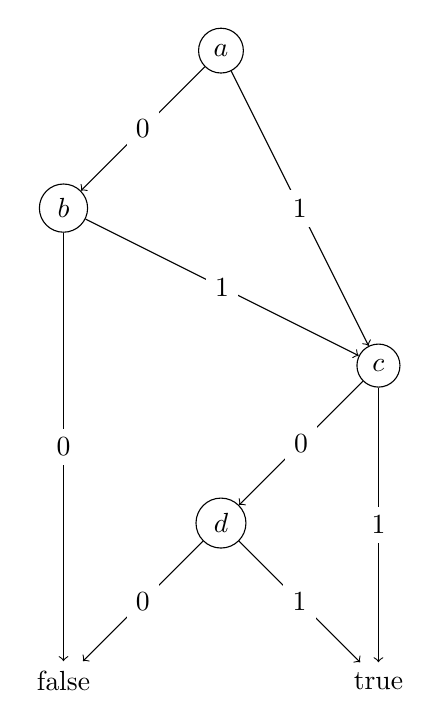
\begin{tikzpicture}[align=center, xscale=2, yscale=2]

\node [circle, draw] (a) at (0, 2) {$a$};
\node [circle, draw] (b) at (-1, 1) {$b$};
\node [circle, draw] (c) at (1, 0) {$c$};
\node [circle, draw] (d) at (0, -1) {$d$};
\node (false) at (-1, -2) {false};
\node (true) at (1, -2) {true};

\draw [->] (a) -- (b) node [midway, fill=white] {0};
\draw [->] (a) -- (c) node [midway, fill=white] {1};
\draw [->] (b) -- (c) node [midway, fill=white] {1};
\draw [->] (b) -- (false) node [midway, fill=white] {0};
\draw [->] (c) -- (true) node [midway, fill=white] {1};
\draw [->] (c) -- (d) node [midway, fill=white] {0};
\draw [->] (d) -- (false) node [midway, fill=white] {0};
\draw [->] (d) -- (true) node [midway, fill=white] {1};

\end{tikzpicture}
\caption{Binary decision diagram for $(a \lor b) \land (c \lor d)$}
\label{fig:bdd}
\end{figure}

\paragraph{Data-flow analysis}

The data-flow analysis represents program as a control flow graph where
nodes are blocks of the program and edges represent the flow of
control. Block is a succession of program instructions where control
enters at the beggining of the block, leaves at the end and does not
branch or halt inside the block. The analysis is executed in two steps:
first a set desired facts is compiled, then the set is used for the
analysis itself \cite{Wogerer05-1}. An example of a control flow graph
with corresponding code can be found in figure \ref{fig:dfg}.

This technique is typically used by compilers to optimize the code. It
can help with detecting constant propagation, common subexpression
elimination or redundant operations \cite{Kildall73-1}. However, it is
not powerful enough to provide detailed information that could be used
to prevent runtime errors due to ommiting the program sematics by usage
of blocks.

\begin{figure}[h]
\centering
\begin{tikzpicture}[align=center]



\end{tikzpicture}
\caption{Data flow graph and corresponding code}
\label{fig:dfg}
\end{figure}

\paragraph{Symbolic execution}

The basic idea is to use symbolic variables instead of the real ones.
For instance, one such usage can be observed in figure \ref{fig:se}.
Throughout the process of symbolic execution SMT solver checks whether
a certain formula is satisfied. TODO citation

The main disadvantage of this approach is scalability -- a symbolic
execution of moderately complex program can lead to large number of paths
that need to be checked. That being said, the continuous evolution in
algorithm design and computer performance mitigate this problem.

\begin{figure}[h]
\begin{minipage}{0.3\textwidth}
\begin{lstlisting}[numbers=left]
a = a + b;
b = a - b;
a = a - b;
\end{lstlisting}
\end{minipage}
\begin{minipage}{0.7\textwidth}
\begin{tabular}{c|c|c}
line & $a$                       & $b$ \\
\hline
1    & $a + b$                   & $b$ \\
2    & $a + b$                   & $(a + b) - b$ \\
3    & $(a + b) - ((a + b) - b)$ & $(a + b) - b$ \\
\hline
final values & $b$             & $a$ \\
\end{tabular}
\end{minipage}
\caption{Sample code and corresponding symbolic execution}
\label{fig:se}
\end{figure}

\paragraph{Abstract interpretation}

The abstract interpretation is described in detail in section
\ref{sec:abstractinterpretation}.


\section{Abstract interpretation}
\label{sec:abstractinterpretation}

The abstract interpretation falls into the category of software
verification by static analysis. It was first defined by P. Cousot and
and R. Cousot in 1977 \cite{CousotCousot77-1}:

\begin{definition}
Abstract interpretation of program consists of using denotations of
computations in some universe of objects to describe computations in
another universe of abstract objects, so that the results of abstract
execution give some informations on the actual computations.
\end{definition}

The key concept here is abstraction. An \textit{abstraction} is a property
of an object that is being analyzed. In figure \ref{fig:abstraction}
there are several abstractions of number 8. This number is positive,
integer, real and rational number. Every one of these abstractions comes
at a cost of precision. The greater the abstraction is the greater is the
loss of precision. Still, an abstraction is often easier to reason about,
mainly in terms of memory -- rather than keeping an enumeration of all
possible values of a number, only an abstraction is kept in memory.

Number 8 from this example represents a \textit{concrete} value. It is
the value that is used during the actual computation.

\begin{figure}[h]
\centering
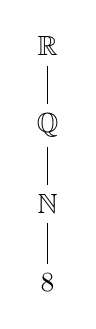
\begin{tikzpicture}[align=center]

\node (real) at (0, 3) {$\mathbb{R}$};
\node (rational) at (0, 2) {$\mathbb{Q}$};
\node (natural) at (0, 1) {$\mathbb{N}$};
\node (eight) at (0, 0) {8};

\draw (real) -- (rational);
\draw (rational) -- (natural);
\draw (natural) -- (eight);

\end{tikzpicture}
\caption{Various abstractions of number 8}
\label{fig:abstraction}
\end{figure}

The shift from concrete value to abstraction is done with
\textit{abstraction function}. This function maps concrete values to
abstract properties of interest. It is traditionally denoted as
$\alpha$.

definition

example

Complementary to the abstraction function is \textit{concretization
function}. It is usually denoted as $\gamma$. It performs a mapping from
abstract values to concrete values. This function is incomplete.

definition

example

Naturally, operations on concrete values need to be somehow transformed
in order to function on abstract values. Such transformed operation is
called \textit{abstract operation}.

example

Lattice

Concrete values are organized in \textit{concrete domain}. Formally,
the concrete domain is a complete lattice $L$:

\begin{align*}
L = \langle \mathcal{P} (A), \subseteq, \emptyset, A, \cap, \cup \rangle
\end{align*}

where $\mathcal{P} (A)$ is power set of $A$. An example of such lattice
for set $A = \{ 1, 2, 3 \}$ can be found in figure
\ref{fig:concretedomain}.

\begin{figure}[h]
\centering
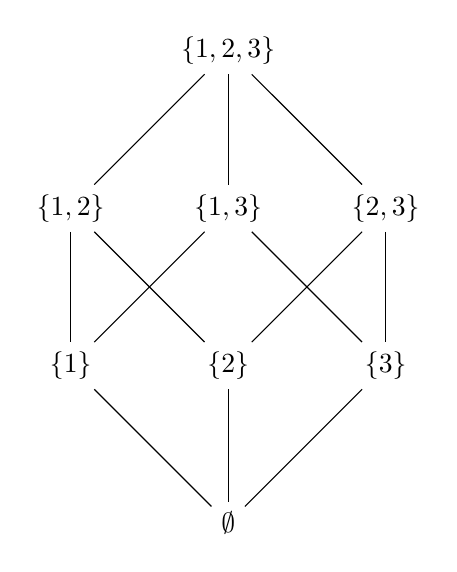
\begin{tikzpicture}[align=center, xscale=2, yscale=2]

\node (123) at (0, 3) {$\{ 1, 2, 3 \}$};
\node (12) at (-1, 2) {$\{ 1, 2 \}$};
\node (13) at (0, 2) {$\{ 1, 3 \}$};
\node (23) at (1, 2) {$\{ 2, 3 \}$};
\node (1) at (-1, 1) {$\{ 1 \}$};
\node (2) at (0, 1) {$\{ 2 \}$};
\node (3) at (1, 1) {$\{ 3 \}$};
\node (empty) at (0, 0) {$\emptyset$};

\draw (123) -- (12);
\draw (123) -- (13);
\draw (123) -- (23);
\draw (12) -- (1);
\draw (12) -- (2);
\draw (13) -- (1);
\draw (13) -- (3);
\draw (23) -- (2);
\draw (23) -- (3);
\draw (1) -- (empty);
\draw (2) -- (empty);
\draw (3) -- (empty);

\end{tikzpicture}
\caption{Concrete domain for set $\{ 1, 2, 3 \}$}
\label{fig:concretedomain}
\end{figure}

Abstract properties are encoded in modules with data structures called
\textit{abstract domain}. This module is a set of all abstract values
for given abstraction. Formally, abstract domain forms a complete
lattice $L'$:

\begin{align*}
L' = \langle \bar{A}, \leq, \bot, \top, \sqcup, \sqcap  \rangle
\end{align*}

Consider the abstraction of positive and negative numbers on set of real
numbers $\mathbb{R}$. The abstract domain for this abstraction is displayed
in figure \ref{fig:abstractdomain}.

\begin{figure}[h]
\centering
\begin{tikzpicture}[align=center]

\node (top) at (0, 3) {$\top$};
\node (negative) at (-1, 2) {$(-)$};
\node (positive) at (1, 2) {$(+)$};
\node (zero) at (0, 1) {$0$};
\node (bottom) at (0, 0) {$\bot$};

\draw (top) -- (negative);
\draw (top) -- (positive);
\draw (negative) -- (zero);
\draw (positive) -- (zero);
\draw (zero) -- (bottom);

\end{tikzpicture}
\caption{Abstract domain for positive and negative numbers on $\mathbb{R}$}
\label{fig:abstractdomain}
\end{figure}

fixpoint?

formal definition of AI

Abstract interpretation promises better scalability when compared to other
methods such as model checking or symbolic execution. It tries to achieve
this through appropriate abstraction choice.


\chapter{Solution design}
\label{chap:design}

This chapter describes strings and three approaches that have been designed
to analyze strings within abstract interpretation framework. Strings play
an important role in day-to-day computer programming. Nowadays, they are
an essential part of every major programming language.


\section{Strings}
\label{sec:strings}

Strings of characters are widely employed in software engineering. They
represent basic building blocks in dynamically typed languages such as
Python, Ruby or Perl. Their usages include expressions of values,
arguments, commands or even whole pieces of code. Strings are frequently
used during generating an output such as XML file or processing an input
in text form. The format of the processed string is often verified by
another part of the system which takes this string as an input, for
instance the format of a SQL query is verified by SQL server processor
which can cause unexpected errors. Moreover, a user might supply a
malicious input when deliberately trying to cause similar effect.
Therefore, it is useful to know how string is formatted and manipulated
during the execution of a program.

The following definitions are describe strings and their properties
formally \cite{Kozen97-1}:

\begin{itemize}

\item An \textit{alphabet} is any finite set. For example an alphabet for
binary numbers is $\{0, 1\}$. It is typically denoted as $\Sigma$. Elements
of alphabet are called \textit{symbols} or \textit{letters} and are denoted
by $a, b, c, \dots$.

\item A \textit{string} over $\Sigma$ is any finite sequence of symbols of
$\Sigma$. For $\Sigma = \{a, b\}$ an example of string is $aabab$. Strings
are denoted by $x, y, z, \dots$.

\item The \textit{length} of a string $x$ is the number of symbols in $x$.
It is denoted as $|x|$. For example, $|aabab| = 5$.

\item \textit{Empty string} is a string with length of 0. It is also called
\textit{null string} and is denoted by $\varepsilon$. Formally,
$|\varepsilon| = 0$.

\item \textit{Concatenation} is an operation which takes two strings $x$
and $y$ and chains them together to form a new string $xy$. It is
associative operation but it not comutative. Empty string $\varepsilon$ is
identity for concatenation. The length of resulting string is a sum of
lengths of concatenated strings.

\begin{align*}
(xy)z &= x(yz) \\
xy &\neq yx \\
\varepsilon x = x \varepsilon &= x \\
|xy| &= |x| + |y|
\end{align*}

\item A \textit{prefix} of a string $x$ is a string $y$ for which there
exists a string $z$ such that $x = yz$. The empty string $\varepsilon$ is
a prefix of every string. String $aaba$ is a prefix of $aababb$. A prefix
$y$ of $x$ is a \textit{proper} prefix of $x$ when $y \neq \varepsilon$ and
$y \neq x$.

\item A \textit{suffix} of a string $x$ is a string $z$ for which there
exists a string $y$ such that $x = yz$. The empty string $\varepsilon$ is
a suffix of every string. String $babb$ is a suffix of $aababb$. A suffix
$z$ of $x$ is a \textit{proper} suffix of $x$ when $z \neq \varepsilon$ and
$z \neq x$.

\end{itemize}

In \texttt{C} programming language strings are separated from the rest of
the code by pair of \texttt{"} (double quote) characters. Internally,
they represent a chunk of memory structurally similar to array. In fact,
string is a specific type of array. Generally, an array can contain any
type of data given all the array items have the same type \footnote{In some
languages members of array do not have to be uniformly typed.} and for
string that data type happens to be \texttt{char}. The end of the string is
determined by a special character \texttt{'\textbackslash0'} called NUL.
Strings terminated by such character are usually called null-terminated
strings.

Obviously, strings and arrays are related to each other quite tightly.
Both of them serve as sets of values sequentially stored in memory.
Nonetheless, there is a difference in the information value they represent.
For example, in an array of integers the information value is uniformly
distributed -- every number in the array carries the same weight. On the
other hand, symbols of string do not carry a lot of information just by
themselves. Having three characters \texttt{'v'}, \texttt{'a'} and
\texttt{'r'} separately does not mean a lot, but together they form
a \texttt{"var"} string which might tell a programmer that variable
declaration follows.

The versatility of strings makes it difficult to analyze them in general.
Intuitively, one can feel there is a difference when trying to analyze
string containing an XML document and string containing filepath. They
have different properties. TODO explain


\section{String abstract domains}

The primary goal of domains described in following sections is to
abstract strings so that they provide useful informations about file
paths. Normally, in UNIX-like operating systems such as Linux or Mac OS
the path is represented by a string containing slash \texttt{'/'} characters
and names of folders or files in between them.

As per the definition of abstract domain from section
\ref{sec:abstractinterpretation} the members of lattice need to be
specified for every suggested domain:

\begin{itemize}

\item set $A$ contains abstract values of particular set (prefixes,
suffixes, tries)

\item partial ordering $\leq$ of abstract values in abstract domain

\item least upper bound $\sqcap$ for every pair of abstract values

\item greater lower bound $\sqcup$ for every pair of abstract values

\item top element $\top$

\item bottom element $\bot$

\end{itemize}

Besides that, the operations specific to particular domain need to be
defined. In this case these are based on functions available to programmer.
Obviously, the C standard library provides numerous functions that operate
on strings, but for the purposes of this work concatenation and
substring functions will suffice. (TODO: why?) They are denoted as \textit{concat} and
\textit{substr} respectively.

The \textit{concat} function has two arguments -- strings that need to be
concatenated. The function follows the semantics of concatenation
operation described in section \ref{sec:strings} and returns these two
strings chained together as one. For instance,
$\textit{concat}(\texttt{"geo"}, \texttt{"logy"})$ yields \texttt{"geology"}.

The \textit{substr} function takes three arguments: a string $x$ and two
natural numbers $i$ and $j$ assuming $i < j$. The function returns a
substring of string $x$ from the $i$-th to the $j$-th symbol of the string.
Note that strings are indexed the same way as arrays -- $x[0]$ is the first
symbol of $x$, $x[1]$ is the second and so on. As an example consider the
function $\textit{substr}(1, 4, \texttt{"automatic"})$ which returns
\texttt{"utom"}.


\section{Prefix abstract domain}

The first of the designed abstract domains is the one that approximates
a string by its prefix. It is based of works of Giulia Constantini,
Pietro Ferrara and Agostino Cortesi \cite{Constantini11-1}. This domain
is has simple semantics, thus it provides a good introduction into the
designed abstract domains.

The abstraction used in this case is string prefix as defined in section
\ref{sec:strings}. Common notation for prefix is $abc*$ where $abc$
represents symbols of prefix and $*$ stands for any string, $\varepsilon$
included. The asterisk is present in prefix all the time so it can be
omitted from this notation.

Partial ordering $\leq$ on this domain is defined as:

\begin{align*}
x \leq y \Leftrightarrow
  x = \bot \lor (\forall i \in [0, |y| - 1] :
  |y| \leq |x| \land y[i] = x[i])
\end{align*}

where $y$ is a function which returns a length of string and
$x$ and $y$ are abstract values representing string
prefixes.

Intuitively, prefixes are ordered in a lattice by their length. Prefix
$x$ is smaller than string $y$ if $y$ is a
prefix of $x$ or $x$ is the bottom of the domain $\bot$.
The length of string abstract values decreases as prefixes are closer to
the top element $\top$. The situation is demonstrated in figure
\ref{fig:prefixlattice}.

\begin{figure}[h]
\centering
\begin{tikzpicture}[align=center]

\node (top) at (0, 3) {$\top$};
\node (s) at (0, 2) {s};
\node (sa) at (-2, 1) {sa};
\node (su) at (2, 1) {su};
\node (sax) at (-3, 0) {sax};
\node (sap) at (-1, 0) {sap};
\node (sup) at (1, 0) {sup};
\node (sud) at (3, 0) {sud};
\node (bottom) at (0, -1) {$\bot$};

\draw (top) -- (s);
\draw (s) -- (sa);
\draw (s) -- (su);
\draw (sa) -- (sax);
\draw (sa) -- (sap);
\draw (su) -- (sup);
\draw (su) -- (sud);
\draw (sax) -- (bottom);
\draw (sap) -- (bottom);
\draw (sup) -- (bottom);
\draw (sud) -- (bottom);

\end{tikzpicture}
\caption{Prefix abstract domain}
\label{fig:prefixlattice}
\end{figure}

The least upper bound operator $\sqcap$ is defined as:

\begin{align*}
\sqcap (\mathsf{S_1}, \mathsf{S_2}) =
\begin{cases}
\mathsf{S} & \text{where } \mathsf{S}
  = \textit{prefix}(\mathsf{S_1}, \mathsf{S_2}) \\
\top       & \text{otherwise}
\end{cases}
\end{align*}

where function $\textit{prefix}(\mathsf{S_1}, \mathsf{S_2})$ returns the
longest common prefix of strings $\mathsf{S_1}$ and $\mathsf{S_2}$. For
example, $\textit{prefix}(\texttt{"capture"}, \texttt{"caption"})$ returns
\texttt{"capt"} and for $\textit{prefix}(\texttt{"house"}, \texttt{"car"})$
returns $\varepsilon$.

Simply put, the least upper bound of two strings $\mathsf{S_1}$ and
$\mathsf{S_2}$ is the longest common prefix of these strings. If there is
none, the upper bound is the top element of the lattice $\top$.

In a similar fashion, the greater lower bound operator $\sqcup$ is defined
by:

\begin{align*}
\sqcup (\mathsf{S_1}, \mathsf{S_2}) =
\begin{cases}
\mathsf{S_1} & \text{if } \mathsf{S_1} \leq \mathsf{S_2} \\
\mathsf{S_2} & \text{if } \mathsf{S_2} \leq \mathsf{S_1} \\
\bot         & \text{otherwise}
\end{cases}
\end{align*}

The greater lower bound is the smaller of the two elements and if none
of them is smaller then it is the bottom element $\bot$.

The semantics for \textit{concat} operation is defined as:

\begin{align*}
\textit{concat}(x, y) = x
\end{align*}

where $x$ and $y$ are string prefixes. The \textit{concat} operation of two
prefixes returns the first of the concatenated prefixes since it is the longest
prefix that is surely included in resulting string.

The \textit{substr} operations semantics is defined by:

\begin{align*}
\textit{substr}(i, j, x) =
\begin{cases}
x[i] \dots x[j - 1]   & \text{if } j \leq |x| \\
x[i] \dots x[|x| - 1] & \text{if } j > |x| \land i < |x| \\
\top                  & \text{otherwise}
\end{cases}
\end{align*}

The situation for substring function is not so straightforward.
The \textit{substr} function returns substring from $i$-th to $j$-th symbol
when index $j$ is less than the length of $x$, it returns symbols from
$i$-th index to the end of $x$ if $i$ is less the length of $x$ but $j$
is greater than the string length and it returns $\top$ top element in
all other cases.


\section{Suffix abstract domain}

The second domain is complementary to the domain approximating using
prefixes. It was presented in the same paper \cite{Constantini11-1} as the
prefix domain. It is relatively simple as well.

Abstract values for this domain are represented by string suffixes.
The notation chosen for suffixes is $*abc$ where $abc$ are symbols of
suffix and $*$ any string. The asterisk is left out since it is always
there.

Partial order $\leq$ for suffixes $x$ and $y$ is:

\begin{align*}
x \leq y \Leftrightarrow
  x = \bot \lor (\forall i \in [0, |y| - 1] : |y| \leq |x| \land
    y[i] = x[i + |x| - |y|])
\end{align*}

For better illustration, the figure \ref{fig:suffixlattice} shows an
example of suffix abstract domain with such order.

\begin{figure}[h]
\centering
\begin{tikzpicture}[align=center]

\node (top) at (0, 3) {$\top$};
\node (n) at (0, 2) {n};
\node (on) at (-2, 1) {on};
\node (un) at (2, 1) {un};
\node (ion) at (-3, 0) {ion};
\node (ton) at (-1, 0) {ton};
\node (sun) at (1, 0) {sun};
\node (fun) at (3, 0) {fun};
\node (bottom) at (0, -1) {$\bot$};

\draw (top) -- (n);
\draw (n) -- (on);
\draw (n) -- (un);
\draw (on) -- (ion);
\draw (on) -- (ton);
\draw (un) -- (sun);
\draw (un) -- (fun);
\draw (ion) -- (bottom);
\draw (ton) -- (bottom);
\draw (sun) -- (bottom);
\draw (fun) -- (bottom);

\end{tikzpicture}
\caption{Suffix abstract domain}
\label{fig:suffixlattice}
\end{figure}

The least upper bound $\sqcap$ is:

\begin{align*}
\sqcap (x, y) =
\begin{cases}
z    & \text{where } z = \textit{suffix}(x,  y) \\
\top & \text{otherwise}
\end{cases}
\end{align*}

where function \textit{suffix} returns the longest common suffix of the
two strings $x$ and $y$. If these strings have common suffix then the least
upper bound is their longest common suffix. Otherwise it is the top
element $\top$.

The greater lower bound is defined as:

\begin{align*}
\sqcup (x, y) =
\begin{cases}
x    & \text{if } x \leq y \\
y    & \text{if } y \leq x \\
\bot & \text{otherwise}
\end{cases}
\end{align*}

If it is possible to compare the two strings, then it is the smaller of the
two. It is the bottom element $\bot$ for all other cases.

The \textit{concat} operation for suffix domain is the second of the
concatenated strings:

\begin{align*}
\textit{concat}(x, y) = y
\end{align*}

The \textit{substr} operation is unusually simple:

\begin{align*}
\textit{substr}(i, j, x) = \top
\end{align*}

It returns the top element $\top$ for all the possible inputs, because
it is impossible to tell whether indexes $i$ and $j$ are within the
boundaries of the suffix.

An example of the domain usage could be filtering files or directories
based on their extensions.


\section{Trie abstract domain}


\chapter{Implementation}
\label{chap:implementation}

Abstract domains designed in chapter \ref{chap:design} are applied in the
context of \texttt{canal} abstract interpreter. First, the architecture of
the interpreter is described and then the implementation of individual
domains is presented.


\section{\texttt{canal}}

Following the project README file \cite{Klic12-1}, the \texttt{canal}
abstract interpreter is a static analysis tool designed to analyze behavior
of application programs written in C programming language. It focuses
on scalability for large programs and handling of real-world source code.

It is divided into three parts:

\begin{description}

\item[Abstract domains] \hfill \\
These modules cover semantic choices, data
structures, algorithmic aspects and implementation details concerning
analysis. Canal contains abstract domains for integers, floating point
numbers, arrays and strings.

\item[Interpreter] \hfill \\
It iterates through the source code until the analysis
is finished. It manages the state of program analysis consisting of
abstract values.

\item[Operations] \hfill \\
They manage translations of program instructions to
abstract operations defined as part of abstract domains. Interpreter uses
operations to update abstract values stored in analysis state.

\end{description}

The tool is utilizes llvm compiler infrastructure. It provides
a frontend called Clang that contains compilers for C, C++, Objective C and
Objective C++ capable of emitting LLVM bitcode. The bitcode is a platform
independent representation of program that is suitable for static analysis.
There are other static analysis tools that leverage the same idea, namely
klee.

The whole process of analysis is performed in following steps:

\begin{enumerate}

\item compilation of a program that is being analyzed into the llvm bitcode
representation

\item loading of compiled program into the interpreter and initialization
with abstract domains

\item interpretation of loaded program with abstract operations on the
domains

\end{enumerate}

Abstract interpreter itself is implemented in C++. It can be compiled with
g++ compiler from the GNU Compiler Collection.

\texttt{canal} comes with command line tool which allows to step through
the execution of interpretation and inspect variables. In that aspect it
is similar to \texttt{gdb}, a popular GNU debugger project for various
languages \footnote{\url{http://www.gnu.org/software/gdb/}}.

The project is relatively young and as of this moment is in its experimental
stage. That being said, a few programs from GNU core utils project
\footnote{\url{http://www.gnu.org/software/coreutils/}} have been
successfully analyzed by interpreter.


\section{Domain interface in \texttt{canal}}

Since \texttt{canal} abstract interpreter is implemented in C++ it enables
usage of classes. Every domain in it corresponds to single class and
operations on the domain are implemented as methods of particular class.
Most of the operations are domain-specific, but there are a few methods
that are universally required to be implemented in order for abstract
values to form a lattice.

Universal methods are enforced by inheriting from \texttt{Domain} class,
which provides their type definitions. These methods are:

\begin{itemize}

\item join

\item meet

\item equality

\item inclusion

\item set top

\item set bottom

\item is top

\item is bottom

\end{itemize}


\section{String prefix}




\section{String suffix}


\section{String trie}


\chapter{Conclusion}
\label{chap:conclusion}


%% Lists of tables and figures, glossary, etc.
%\printindex
%\printglossary
%\listoffigures
%\listoftables

%% Bibliography
\renewcommand*{\bibname}{\chapter{Bibliography}\vspace{-1em}}
\begin{thebibliography}{99}

\bibitem{CousotCousot77-1}
P{.} Cousot and R{.}Cousot.
\newblock Abstract interpretation: a unified lattice model for static
  analysis of programs by construction or approximation of fixpoints.
\newblock In \emph{Conference Record of the Fourth Annual ACM
  SIGPLAN-SIGACT Symposium on Principles of Programming Languages},
  pages 238--252, Los Angeles, California, 1977. ACM Press, New York,
  NY, USA.

\bibitem{Cousot00-1}
P{.} Cousot.
\newblock Abstract interpretation based formal methods and future
  challenges.
\newblock In \emph{Informatics - 10 Years Back, 10 Years Ahead},
  volume 2000 of LNCS, pages 138--156. Springer, 2000.

\bibitem{Moore65-1}
G{.} E{.} Moore.
\newblock Cramming more components onto integrated circuits.
\newblock In \emph{Electronics}, volume 38, number 8, pages 114--117. 1965.

\bibitem{EmanuelssonNilsson08-1}
P{.} Emanuelsson, U{.} Nilsson.
\newblock A comparative study of industrial static analysis tools (extended
  version).
\newblock In \emph{Electronic Notes in Theoretical Computer Science},
  volume 217, pages 5--21. 2008.

\bibitem{Boulanger12-1}
J{.}--L{.} Boulanger.
\newblock Static Analysis of Software: The Abstract Interpretation.
\newblock Wiley, 2012.

\bibitem{Ernst03-1}
M{.} D{.} Ernst.
\newblock Static and dynamic analysis: Synergy and duality.
\newblock In \emph{Workshop on Dynamic Analysis}, pages 24--27. 2003.

\bibitem{Woodcock09-1}
J{.} Woodcock, P{.} G{.} Larsen, J{.} Bicarregui and J{.} S{.} Fitzgerald.
\newblock Formal methods: Practise and experience.
\newblock In \emph{ACM Computing Surveys}. 2009.

\bibitem{Turing36-1}
A{.} Turing.
\newblock On computable numbers, with an application to the
  Entscheidungsproblem.
\newblock In \emph{Proceedings of the London Mathematical Society},
  pages 230--265. 1936.

\bibitem{Sipser06-1}
M{.} Sipser.
\newblock Introduction to the Theory of Computation (Second Edition).
\newblock Thomson Course Technology, 2006.

\bibitem{Kozen97-1}
D{.} Kozen.
\newblock Automata and Computability.
\newblock Springer, 1997.

\bibitem{Chess04-1}
B{.} Chess, G{.} McGraw.
\newblock Static Analysis for Security.
\newblock In \emph{Security and Privacy, IEEE}, volume 2, number 6,
  pages 76--79, 2004.

\bibitem{Clarke99-1}
E{.} M{.} Clarke, O{.} Grumberg, D{.} A{.} Peled.
\newblock Model checking.
\newblock MIT Press, 1999.

\bibitem{Wogerer05-1}
W{.} W\"{o}gerer.
\newblock A Survey of Static Program Analysis Techniques.
\newblock Available at \url{http://www.ics.uci.edu/~lopes/teaching/inf212W12/readings/Woegerer-progr-analysis.pdf}
  (May 2013).

\bibitem{Kildall73-1}
G{.} A{.} Kildall.
\newblock A Unified Approach to Global Program Optimization.
\newblock In \emph{Proceedings of the 1st annual ACM SIGACT-SIGPLAN
  symposium on Principles of programming}, pages 194--206, 1973.

\bibitem{Constantini11-1}
G{.} Constantini, P{.} Ferrara, A{.} Cortesi.
\newblock Static analysis of string values.
\newblock In \emph{Proceedings of the 13th Internation Conference on Formal
  Engineering Methods}, 2011.

\bibitem{Klic12-1}
K{.} Klíč.
\newblock Canal, abstract intepreter for real-world application programs.
\newblock Available at \url{https://github.com/karelklic/canal/blob/master/README}
  (May 2013).

\end{thebibliography}


%% Additional materials
\appendix

\chapter{Instructions for running \texttt{canal}}
\label{chap:instructions}

%% End of the whole document
\end{document}

